\documentclass{article}
%\documentclass[2pt,english]{article}

\usepackage{cite}
\usepackage{listings}
%\usepackage{times}
\usepackage{color}
\usepackage{url}
\urlstyle{same} % Used for formatting formatting url footnotes
\usepackage{soul} % highlighting
\usepackage{forloop} % Project timeline
\usepackage{tabularx} % table text width
\usepackage{xcolor,colortbl} %%% Color Table Header
\usepackage{fancyhdr} % Header
%\usepackage{framed}		% Allows drawing text boxes
\usepackage{pgfgantt}
\usepackage{enumitem} % Use for enumerating A, B, C etc...

%Use a font size no smaller than 11 point and one inch margins.

\usepackage{xspace} % Needed for et al.
\newcommand{\etal}{{et al.\@\xspace}}

% Addressing Decision-Making Uncertainty in Self-Adaptive Systems By Accounting for Tactic Volatility
% 
\newcommand{\Title}{Reducing Decision-Making Uncertainty in Self-Adaptive Systems By Accounting for Tactic Volatility Using Bayesian Ridge Regression}


%\newcommand{\Title}{Accounting for Tactic and Cost Volatility in Self-Adaptive Systems by Using Dynamic Bayesian Matrix Factorization}

\title{\Title} 


%\title{Reducing Tactic Latency Uncertainty in Self-Adaptive Systems}




\author{
	TPOC: Daniel E. Krutz and Qi Yu; \{dxkvse, qi.yu\}@rit.edu\\
}
 \date{} % Remove the date

% Alter these values based on the actual length.
% The paper should be ~3 pages
%\usepackage[top=.3in, bottom=1in, left=1in, right=1in]{geometry} %% Changes the margins of the pages - This was breaking the header functions

\usepackage[bottom=1in, left=1in, right=1in, top=.3in]{geometry} %% Use this to make the page wider

\newcommand{\todo}[1]{\textcolor{cyan}{\textbf{[#1]}}}
%\newcommand{\XXX}[1]{\textcolor{green}{{\it [XXXX says: #1]}}}
%\newcommand{\XXX}[1]{\textcolor{yellow}{{\it [XXXX says: #1]}}}
\newcommand{\dan}[1]{\textcolor{blue}{{\it [Dan says: #1]}}}
\newcommand{\amit}[1]{\textcolor{red}{{\it [Amit says: #1]}}}
\newcommand{\hiten}[1]{\textcolor{orange}{{\it [Hiten: #1]}}}


\pagestyle{fancy}
\lhead{\Title} % Leave empty to keep sections from being shown
\rhead{Daniel E. Krutz}

\usepackage{lastpage}
%\cfoot{\thepage\ of \pageref{LastPage}}



\begin{document}

\maketitle
\vspace{-10mm}
\section{Introduction}

% Don't make too buzzwordy. Make it so everyone can understand this.
%you need to introduce 'decision making', before you enter into the volatility in decision making. ex-1: Self-adaptive systems autonomously react to changing situations. Decisions are made based on... These decisions frequently contain volatility... ex-2: Self-adaptive systems autonomously react to chanting situations through a set formula for decision making. 



Self-adaptive systems autonomously react to changing situations through tactics (decisions). Example tactics include a cloud activating an additional virtual machine when the workload reaches a defined threshold, or a UAV taking steps to defeat an enemy threat. These tactics frequently contain volatility in the form of the time necessary to perform the action, availability of the action, the dependability of the action and the cost to perform the action. This volatility can substantially impact the decision-making process. Unfortunately, current self-adaptation processes cannot account for this volatility during the decision-making process. This can negatively impact the system's efficiency, resiliency, and ability to complete mission objectives. To address this challenge, \textbf{we present a Tactic Volatility Aware (TVA) approach that accounts for volatility in the decision-making process of self-adaptive/autonomous systems.} This is innovative as existing techniques are unable to consider tactic volatility in the decision-making process.


\section{Motivating Example}

An autonomous UAV is performing an ISR mission, with the objective of collecting information on suspected enemy combatants. The camera has an anticipated preparation time of .2 seconds. However, due to a mechanical issue, it has been taking .4 seconds to prepare the camera. In existing self-adaptive techniques, the system will be unable to learn about this latency volatility from previous experiences, and will be therefore unable to account for this unanticipated additional latency time. Our Tactic Volatility Aware (TVA) process will enable the system to learn from prior experiences and account for this volatility.

%Figure~\ref{fig:UAVLatencyExampleCamera} represents a scenario where 

\begin{figure}[h]
	\centering
    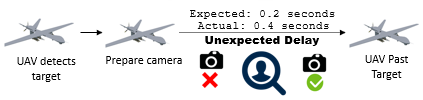
\includegraphics[scale=0.85]{images/UAVLatencyExampleCamera.png}
    \caption{Detrimental Impact of Unexpected Latency Volatility on Autonomous UAV}
    \label{fig:UAVLatencyExampleCamera}
\end{figure}


%For our motivating example, let us consider a scenario of a cloud computing hosting platform that has the goal of providing content to a variable number users. The Service Level Agreement (SLA) defines a maximum threshold $T$ for the average response time, with penalties being incurred for not meeting this response time. When the system predicts that $T$ is going to be surpassed, it should invoke the tactic of adding an additional server resource ($t_1$) to meet the demands of the system. The secondary goal of the system is to minimize operational costs, therefore the system will want to have the minimum number of servers running to satisfy the primary goal of keeping response time $< T$. The process of invoking an additional server resource is not instantaneous, and can have a latency which should be accounted for. Therefore, when the system predicts that $T$ is going to be surpassed, when possible $t_1$ should be invoked with enough time to account for the expected tactic latency, but not too far in advance to ensure that the secondary goal of limiting costs is achieved. In the event that $T$ is impossible to achieve, or that not enough time is available to fully realize the benefits of $t_1$ before $T$ is surpassed, the system may use a \emph{dimmer} function to reduce optional content to ensure that required content is still able to be provided. We will arbitrary assume that the latency of adding a server is expected to be 100 seconds. However, in this scenario the time necessary to add additional server resources has been observed to be consistently $>$ 200 seconds. This will cause the system to execute $t_1$ too late, and could lead to $T$ being surpassed. Conversely, if the the latency time to add a server is observed to be far less than expected, then the system could be using too many resources thus not satisfying the secondary goal of reducing costs. \emph{Therefore, it is imperative to accurately predict tactic volatility to ensure that system goals are met and the maximum award is achieved.}

%\dan{update this}


% ISR mission
% Make this good as we might be able to use it for the FSE paper


% Make sure to also include cost












%% DK: Should the example be more focused on large or small UAVs? - What are they more interested in?
%In this scenario, an autonomous UAV has the objective of collecting information on suspected enemy combatants when they are identified. The camera has an anticipated preparation time of .2 seconds. However, due to a mechanical issue, it has been taking .4 seconds to prepare the camera. In existing self-adaptive techniques, the system will be unable to learn about this latency volatility from previous experiences, and will be therefore unable to account for this unanticipated additional latency time. Our Tactic Volatility Aware (TVA) process will enable the system to learn from prior experiences and account for this volatility.

%Figure~\ref{fig:UAVLatencyExampleCamera} represents a scenario where 

%\begin{figure}[h]
%	\centering
%    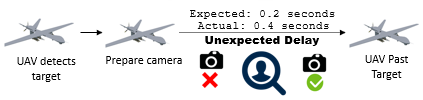
\includegraphics[scale=0.5]{images/UAVLatencyExampleCamera.png}
%    \caption{Impact of Unexpected Latency in UAV}
%    \label{fig:UAVLatencyExampleCamera}
%\end{figure}

\vspace{-3mm}
\section{Proposed Tactic Volatility Aware (TVA) Solution}

%\begin{enumerate}[noitemsep]
%	\item Remedy inaccurate decision volatility determinations made by humans.
%    \item Enable systems to make more accurate decisions, leading to more resilient autonomous devices that are better suited to complete desired mission objectives.

%    \item Ability to update the expected decision volatility values through observing decision-making variability in the system.
%    \item Enable system to account for cost volatility

%	\item Increases the resiliency of the system as it will be able to learn from prior experiences and avoid tactics that lead to undesirable outcomes. 
%	\item Instead of only considering the \emph{utility (benefit)} of executing a tactic, the proposed process makes tactic \emph{cost} a first-class concern. Considering cost provides a more comprehensive decision-support perspective in comparison with existing techniques.

%\end{enumerate}

%\dan{some of these are redundant}


We will develop a {\bf Bayesian dynamic matrix factorization model} to predict tactic volatility. This model will use prior tactic observations to predict future tactic volatility. Our Tactic Volatility Aware (TVA) solution will be easy to incorporate into popular self-adaptation loops such as MAPE-K, making it readily adoptable by a wide variety of autonomous devices, ranging from small cyber physical systems to large UAVs. TVA will offer several advantages over existing decision-making systems that are unable to consider real-world tactic volatility:

%We will develop a {\bf Bayesian dynamic matrix factorization model that jointly predicts multiple correlated tactic volatility parameters}, including cost, latency, dependability, and availability. The joint prediction model assumes that there are a number of common factors, including both observable and latent, that affect these parameters. However, they may play a different role over different parameters. We will begin by modeling the latent factors and their contribution to the parameter of interest. 

%Our Tactic Volatility Aware solution will be easy to incorporate into popular self-adaptation loops such as MAPE-K, making it readily adoptable by a wide range of autonomous devices. Our Tactic Volatility Aware solution offers several advantages over existing decision-making systems that are unable to consider real-world tactic volatility:

\begin{enumerate}[noitemsep]
	\item Remedy inaccurate decision volatility determinations made by humans.
    \item Enable systems to make more accurate decisions, leading to more resilient autonomous devices that are better suited to complete desired mission objectives.
 %   \item Account for variations in volatility through calculated standard deviation in observed tactics.
	\item Improve system predictability.
%	\item Instead of merely considering the benefit of executing a tactic, the proposed process makes tactic \emph{cost} a first-class concern. Considering cost provides a more comprehensive decision-support perspective in comparison with existing techniques.
%	\item Enable systems to complete mission and safety critical operations by accounting for tactic volatility.
%    \item Ability to update the expected decision volatility values through observing decision-making variability in the system.
%	\item Enable human engineer to define the maximum allowed decision-making latency to protect against decision latency that is outside of the defined maximum threshold.
\item Enable system to avoid tactics that may be outside of the desired threshold, or may have unacceptable levels of volatility.


\end{enumerate}




\end{document}





